\clearpage

\def\chaptertitle{Performance Evaluation}

\lhead{\emph{\chaptertitle}}

\chapter{\chaptertitle}
\label{ch:performance-evaluation}

In this chapter, we begin by discussing the underlying hardware configuration, and assumptions made before beginning the auto-scaling experiments in section \ref{sec:ch5-hardware-assumptions}. The cluster configuration, which involves the resource divisions between servers, overall cluster architecture, and deployment resources is discussed in section \ref{sec:ch5-cluster-config}.

\section{Assumptions and Underlying Hardware}
\label{sec:ch5-hardware-assumptions}

For the hardware setup, servers in the Melbourne Research Cloud \footnote{\url{https://docs.cloud.unimelb.edu.au/}} were leveraged to deploy microservices on. The set up consisted of 6 servers, using a total of 16 CPU cores and 48GB of memory. These servers were separated into a cloud and edge layer. The servers on the cloud layer have a significantly higher amount of CPU cores and memory assigned compared to the servers in the edge layer, to simulate the scarcity of resources in the edge layer. Furthermore, a simulated latency was added between inter-layer server communication to mimic the perceived distance between edge nodes and large data-centres.\par

Each server consists of an Ubuntu 22.04 operating system. Kubernetes v1.28.2 is used as the container orchestration technology behind the experimental micro service setup. For maximum flexibility, a bare-metal implementation of Kubernetes is used, instead of ready made solutions available from Amazon or Google. The control plane is deployed on the cloud layer, while the data plane is on the edge layer. Furthermore, several assumptions were made before proceeding with the experimentation:

\begin{itemize}
    \item The only auto-scaling performed would be horizontal pod auto-scaling. Vertical and cluster auto-scaling were out of scope of the project.
    \item The pods on which auto-scaling are not applied will have the maximum possible resource allocation to remove the chances of bottleneck.
    \item At no point in the experiment would a node be taken down, or new node be added.
    \item The autoscaler assumes that every node in the edge layer is an equally likely candidate for scheduling pods on.
\end{itemize}

\section{Cluster Configuration}
\label{sec:ch5-cluster-config}

The hardware was divided into the cloud and edge layer as depicted in table \ref{tab:cluster-hw-overview}. The control plane was divided into two servers, one for handling the Kubernetes control plane scheduling, API service, and etcd deployments, and the other for storing the Prometheus database, along with the microservice Jaeger metrics collection. The edge layer consisted of four servers with far less resources, to depict the difference in computing power. The network layer between the edge and cloud deployments also contained a simulated latency to denote the perceived geographical distance between them.\par

%TC:ignore
\begin{table}
    \caption{Cluster architectural layout}\label{tab:cluster-hw-overview}
    \centering
    \begin{tabular}{|l|l|l|l|}
        \hline
        Node & Layer & CPU (cores) & Memory (GB)\\
        \hline
        Control-Plane-K8s & Cloud & 4 & 16\\
        Control-Plane-DB  & Cloud & 4 & 16\\
        Data-Plane-1      & Edge  & 2 & 4\\
        Data-Plane-2      & Edge  & 2 & 4\\
        Data-Plane-3      & Edge  & 2 & 4\\
        Data-Plane-4      & Edge  & 2 & 4\\
        \hline
    \end{tabular}
\end{table}
%TC:endignore

The cloud and edge nodes were differentiated in through Kubernetes through the internal labelling system. A key ``type'' with value either ``cloud'' or ``edge'' was added to each node. This would enable the scheduler to automatically consider restricting the deployment of pods to particular nodes. For example, the Prometheus deployment would only be deployed on the node of type cloud. This process is known as ``node affinity'' \cite{santos2019towards}.\par

There were several options to deploy the social media application to Kubernetes. Manually cloning them from the repository, creating the custom resource definitions (CRDs), and deploying the YAML files is an option which gives maximum flexibility, but is difficult to debug if things go wrong. Due to this, the Kubernetes package manager Helm was used. Helm \footnote{\url{https://helm.sh/}} is another open-source project whose primary goal involved streamlining the installation, maintenance, and removal of Kubernetes deployments. This is achieved through the use of a Helm chart, which details the configuration of the project, and how to update and access it.\par

Therefore the social media application was the first to be deployed on Kubernetes. However, before deploying the application, the primary deployments to be tested needed to be configured. Based on the ``wrk2'' benchmark that was discussed above, two APIs were identified. One was a GET call to the user's home timeline, and the other was a POST method made by the user to create a post.\par

First, a default social media deployment was installed using the helm command below:

\begin{lstlisting}[
  caption={Social network installation using Helm},
  captionpos=t,
  label={lst:social-network-helm-install},
  language=bash
]
$ helm install social-media \
/DeathStarBench/socialNetwork/helm-chart/Chart.yaml -n default
\end{lstlisting}

With the social media network now deployed, a workload for both GET and POST commands were invoked to generate the latency trace on Jaeger, as depicted in listing \ref{lst:wrk2-api-calls}.

\begin{lstlisting}[
  caption={Social network installation using Helm},
  captionpos=t,
  label={lst:wrk2-api-calls},
  float=ht,
  language=bash
]
$ WRK2="/DeathStarBench/wrk2/wrk -D exp -t 1 -c 1 -d 1 -L -s -R 1"
$ HT=./wrk2/scripts/social-network/read-home-timeline.lua
$ CS=./wrk2/scripts/social-network/compose-post.lua
$ IP=$(kubectl get svc nginx-thrift --template '{{.spec.clusterIP}}')
$ PORT=8080
$ $WRK2 $HT http://$IP:$PORT/wrk2-api/home-timeline/read
$ $WRK2 $HT http://$IP:$PORT/wrk2-api/post/compose
\end{lstlisting}

With the traces generated, the deployments which require autoscaling could be identified for each. From the Jaeger traces generated in figure \ref{fig:ht-cp-trace}, it is clear that the two deployments highlighted in purple, namely ``home-timeline-service'', and ``compose-post-service'', were the major bottlenecks in API processing, and thus required autoscaling. Therefore, the helm deployment was updated to assign resources to them. The resources were assigned in a realistic manner consistent with edge deployments, and based on the number of components each deployment answered to. Listing \ref{lst:deploy-resource-update} shows the CPU resources assigned to both deployments.\par

\begin{figure}[htb]
    \centering
    \caption{Home Timeline and Compose Post API trace}
    \label{fig:ht-cp-trace}
    \begin{minipage}{0.25\linewidth}
        %\caption{Home Timeline API trace}
        %\label{fig:home-timeline-trace}
        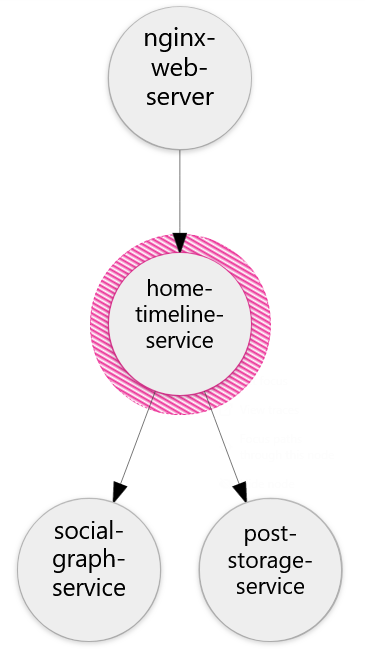
\includegraphics[width=1.0\linewidth]{Figures/Home-Timeline-GET-Trace.png}
    \end{minipage}\hfill
    \begin{minipage}{0.75\linewidth}
        %\caption{Compose Post API trace}
        %\label{fig:compose-post-trace}
        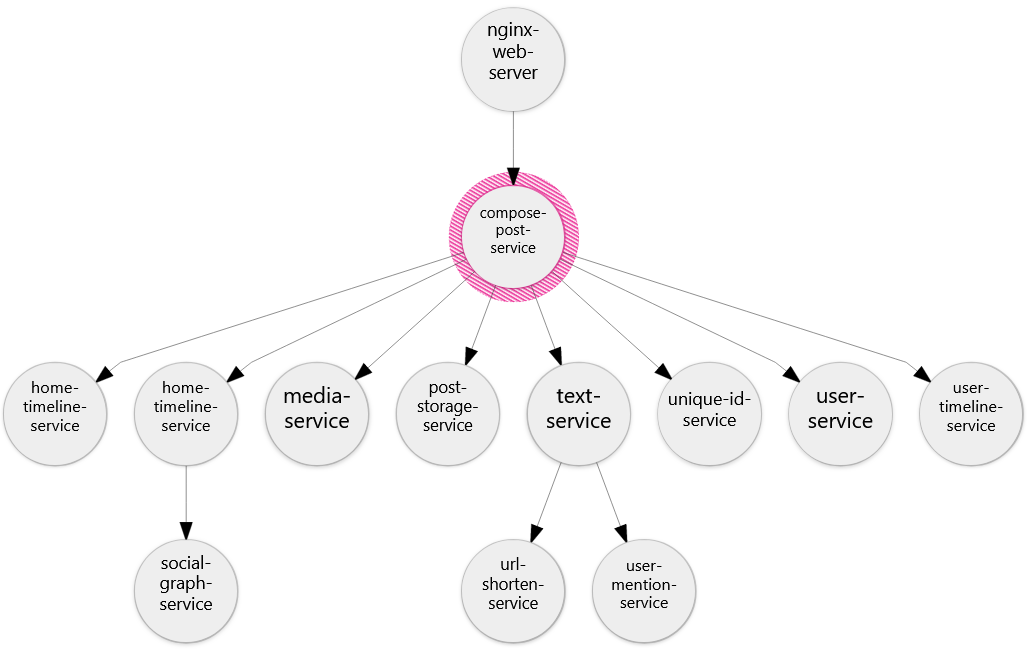
\includegraphics[width=1.0\linewidth]{Figures/Compose-Post-POST-Trace.png}
    \end{minipage}
\end{figure}

\begin{lstlisting}[
  caption={Update resources for bottlenecked deployments},
  captionpos=t,
  label={lst:deploy-resource-update},
  language=bash
]
$ helm upgrade social-media \
/DeathStarBench/socialNetwork/helm-chart/Chart.yaml -n default \
--set-string compose-post-service.container.resources="requests: 
      cpu: "30m"
    limits:
      cpu: "30m"" \
--set-string home-timeline-service.container.resources="requests: 
      cpu: "15m"
    limits:
      cpu: "15m""
\end{lstlisting}

\section{Experiment Setup}
\label{sec:ch5-exp-setup}

Two independent experiments were conducted to verify the performance of the hybrid autoscaler. The social media application was first tested using the GET API to autoscale the home-timeline-service deployment. Then, a more demanding as well as challenging workload was applied to the POST API for autoscaling the compose-post-service deployment. For both these experiments, the workload generation algorithm was used to create realistic daily workloads and tested over the period of one week. Both experiments would configure a flexible SLA latency agreement to be maintained. For the first experiment, the SLA constraint was set to a 150 milliseconds latency, and for the second experiment, it was 1000 milliseconds. The flexible SLA constraint was the primary focus of the experiment, however a moderate and strict SLA constraint was also chosen and tested. The SLA values are shown in table \ref{tab:experiment-sla-values}.\par

%TC:ignore
\begin{table}
    \caption{Experimental SLA constraints}\label{tab:experiment-sla-values}
    \centering
    \begin{tabular}{|l|l|l|}
        \hline
        SLA Type & GET API constraint (ms) & POST API constraint (ms)\\
        \hline
        Flexible    & 150   & 1000\\
        Moderate    & 125   & 900\\
        Strict      & 100   & 800\\
        \hline
    \end{tabular}
\end{table}
%TC:endignore

For the proposed hybrid algorithm to achieve these autoscaling goals within the SLA constraints, the autoscaling subsystems were configured as follows. The reactive autoscaler would check if the CPU utilization of the deployment was exceeding the 50\% threshold. If so, it would scale up based on the cooldowns and tolerations set. The proactive autoscaler on the other hand would check if the forecasted CPU utilization in the next 20 minutes was going to breach the 50\% threshold, and if so, would autoscale with the same configured parameters as the reactive one. The daemon would store the total CPU utilization of the deployment as a time-series for a maximum of seven days, and constantly check for SLA violations to tweak the hyper-parameters of the forecaster as discussed above in section \ref{subsec:ch4-auto-daemon-subsection}. To measure the effectiveness of the hybrid autoscaler, three baseline algorithms were chosen for comparison. All three would autoscale at the CPU threshold of 50\%. Furthermore, these algorithms would be implementations based on the ones discussed in section \ref{sec:ch2-lit-review}.\par

The first was the default Kubernetes horizontal pod autoscaler. No modifications to the configuration were made, thus the scale up cooldown was 0 seconds, while the scale down was 300 seconds. Additionally, the autoscaler had no knowledge of the workload distribution or SLA violations on the edge nodes.\par

The second baseline was an implementation of the reactive traffic aware horizontal pod autoscaler created by Phan et al. \cite{phan2022traffic}. This autoscaler scheduler would compute the ratio of workloads being exerted on the different edge nodes with the deployment pods. Once it did so, it would scale these resources in a commensurate proportion.\par

Finally, the last baseline implementation was the Proactive Pod Autoscaler (PPA) devised by Ju et al. \cite{ju2021proactive}. This algorithm was an open-ended implementation which enabled the user to plugin a deep learning model of their choice. The PPA architecture consisted of three sub-sections, the formulator, evaluator, and updater. An LSTM model was injected into the autoscaler as the model file. This LSTM implementation was similar to the one used in the hybrid autoscaler, however it differed in two key elements. First, the LSTM did not expect pre-processed data without noise, and thus dealt with more complex time-series data. Secondly, due to this additional computation, the LSTM contained a deeper architecture layer with more neural network units. This was required as the algorithm had to correctly predict the complete future workload since there was no reactive autoscaler to fall back on. Over a fixed interval, the algorithm continuously looped through the time-series data and saved the forecast result to a metrics file. The evaluator took these outputs from the metrics file, along with the LSTM from the model file to predict the number of pods to assign in advance, and requested the Kubernetes scheduler for scaling through the API Service. A second loop, known as the update loop, then updated the LSTM model using the latest forecast, and cleared the metrics file. The hyper-parameters were carefully tuned to ensure that the model did not under-perform too significantly. Finally, the PPA architecture did not take into account SLA compliance, and thus SLA metrics were not provided as a feedback for hyper-parameter tuning.\par


